\section{Speech Experiments}
\label{section:speech}

We perform experiments to study a compositional approach of integrating speech capabilities into Llama 3, resembling the method we used for visual recognition. On the input side, an encoder, together with an adapter, is incorporated to process speech signals. We leverage a system prompt (in text) to enable different modes of operation for speech understanding in Llama 3.
If no system prompt is provided, the model acts as a general-purpose spoken dialogue model which can effectively respond to the user speech in a manner that is consistent with the text-only version of Llama 3.
The dialogue history is introduced as the prompt prefix to improve the multi-round dialogue experience.
We also experiment with system prompts that enable the use of Llama 3 for automatic speech recognition (ASR) and automatic speech translation (AST).
The speech interface of Llama 3 supports up to 34 languages.\footnote{The speech interface supports the following 34 languages:
	Arabic,
	Bengali,
	Chinese,
	Czech,
	Dutch,
	English,
	Finnish,
	French,
	German,
	Greek,
	Gujarati,
	Hindi,
	Hungarian,
	Indonesian,
	Italian,
	Japanese,
	Kannada,
	Korean,
	Malayalam,
	Marathi,
	Persian,
	Polish,
	Portuguese,
	Romanian,
	Russian,
	Spanish,
	Swahili,
	Swedish,
	Tamil,
	Telugu,
	Thai,
	Turkish,
	Urdu,
	Vietnamese.}
It also allows for the interleaved input of text and speech, enabling the model to solve advanced audio-comprehension tasks.

We also experiment with a speech generation approach in which we implement a streaming text-to-speech (TTS) system that generates speech waveforms on-the-fly during language model decoding. We design the speech generator for Llama 3 based on a proprietary TTS system and do not fine-tune the language model for speech generation. Instead, we focus on improving speech synthesis latency, accuracy, and naturalness by leveraging Llama 3 embeddings at inference time.
The speech interface is illustrated in Figure~\ref{sph:fig:multimodal_model_overview} and~\ref{sph:fig:model}.

\begin{figure}
    \centering
    
\includegraphics[width=\textwidth]{assets/llama-speech-6x.png}
    \caption{\textbf{Architecture of our speech interface for Llama 3.}}
    \label{sph:fig:model}
\end{figure}

% \section{Center Embedding Leads to The Hierarchical Rule}
\section{Data Complexity Determines Rule Preference}
\label{sec:data_complexity}

We find that models generalize hierarchically because they are trained on data which includes center embeddings, a linguistic structure which we describe in Section \ref{sec:center_embed}. Center-embedded sentences drive hierarchical generalization in both the QF task (Section \ref{sec:qf_result}) and the TI task (Section \ref{sec:ti_result}).

\begin{figure}[t!]
    \centering
    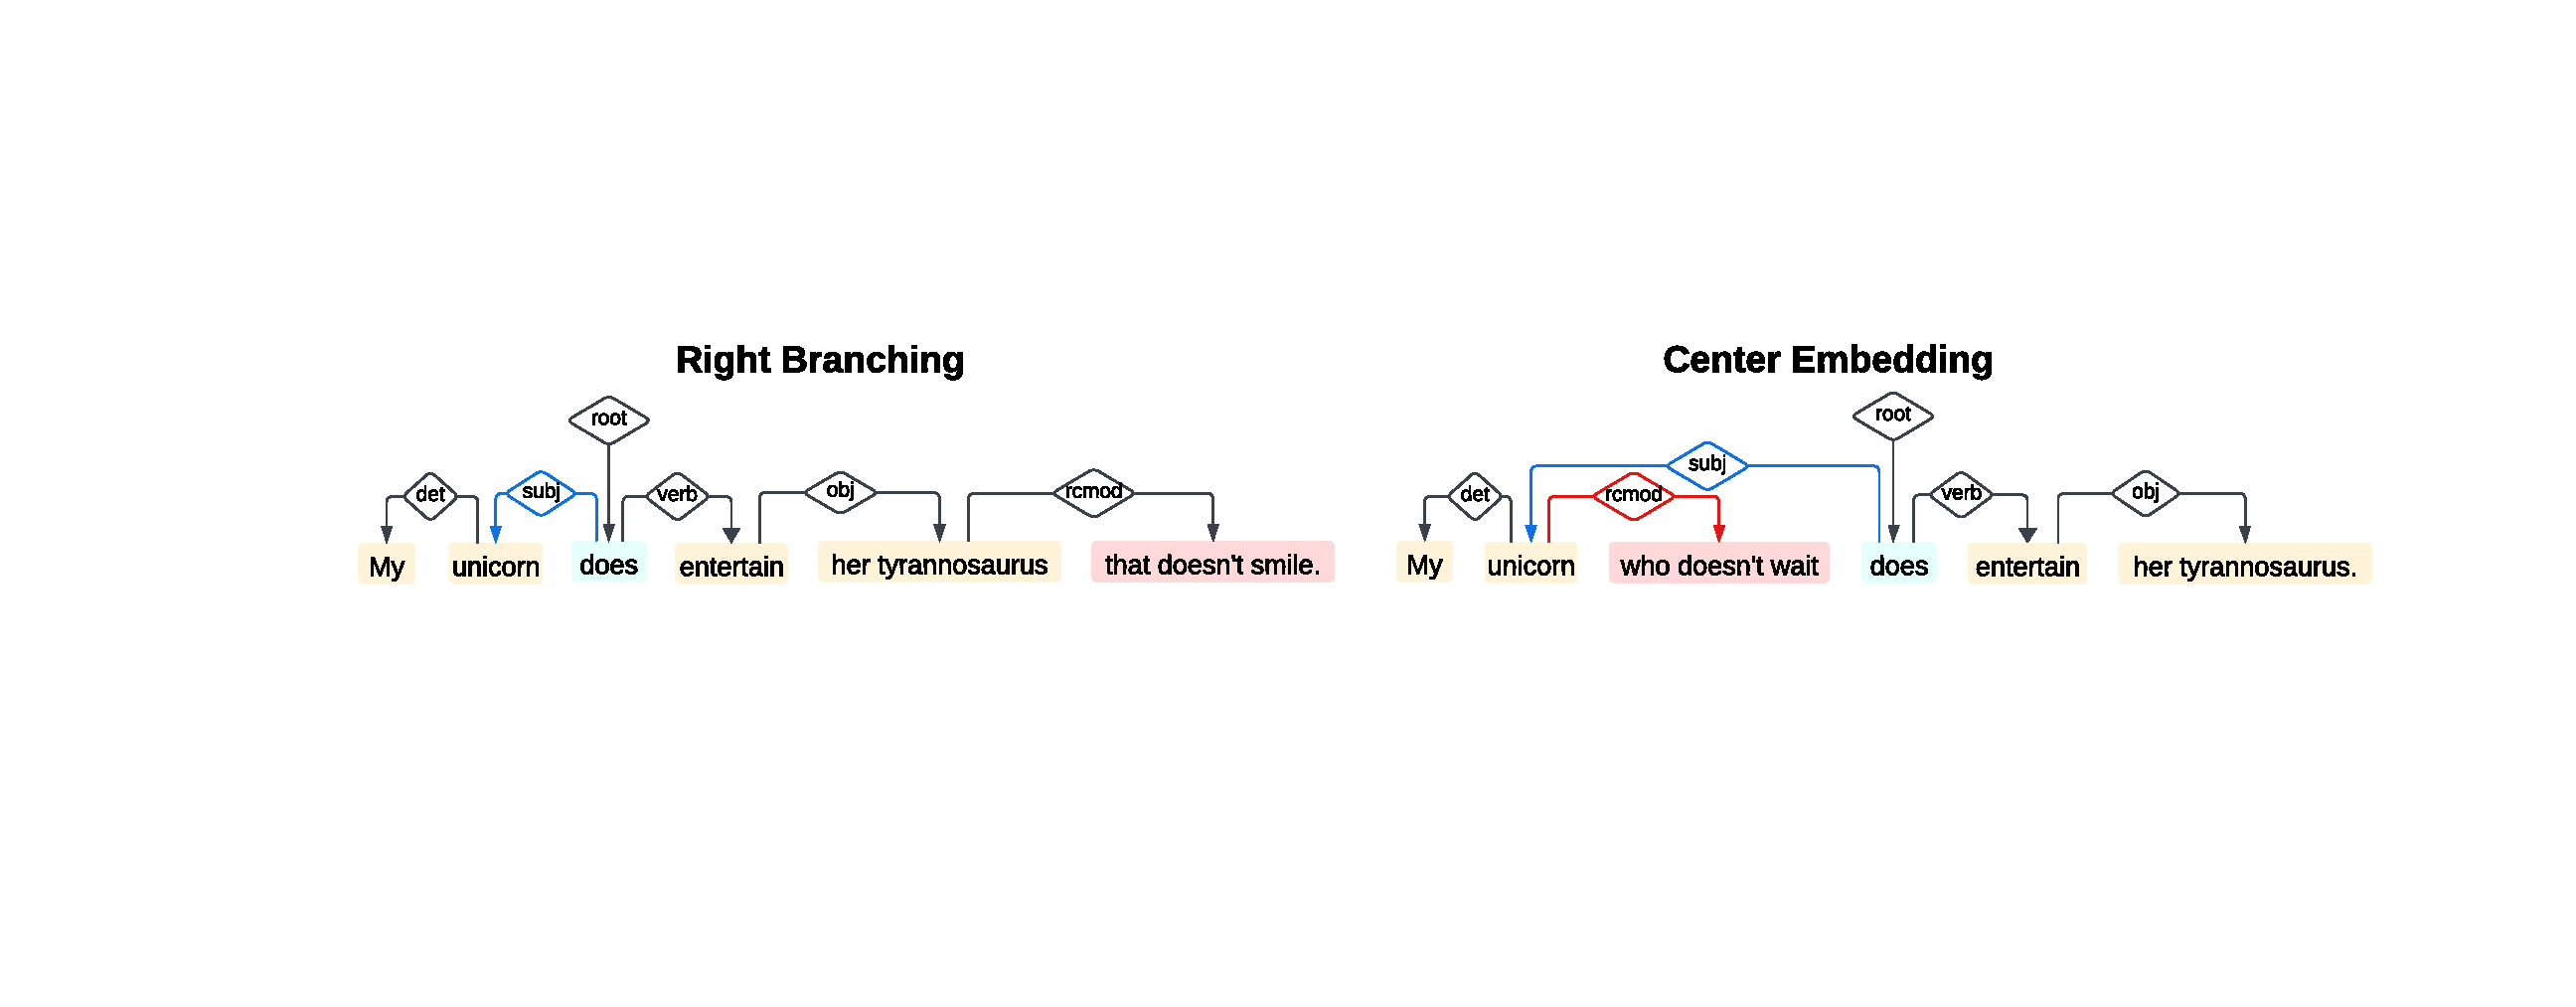
\includegraphics[width=1.0\textwidth]{figures/sentence_demo.pdf}
    \caption{\textbf{Sentence Examples.}   \textit{Left:} Right-branching sentence example. The linear progression of the main constituent is not interrupted by the relative clause. 
    \textit{Right:} Center-embedded sentence example. When the relative clause modifies the subject, it interrupts the linear progression of the main constituent. 
    }
    \label{fig:sentence_demo}
\end{figure}

\subsection{Center Embedding}
\label{sec:center_embed}
Center embedding occurs when a clause is placed recursively within another clause of the same type. Figure \ref{fig:sentence_demo} (\textit{left}) illustrates two examples of center-embedded sentences, where the embedded clause complicates syntactic parsing by placing an additional subject noun in between a verb and its own subject. Whereas center embeddings exhibit a recursive structure, sentences without center embeddings are exclusively right-branching. Right-branching structures may also include modifying clauses, but these clauses can only be appended at the end of the main clause, maintaining its linear flow (see Figure \ref{fig:sentence_demo}, \textit{right}). Linguists have long argued that center embeddings play a crucial role in grammar acquisition \citep{wexler1980formal} and give rise to tree-like syntactic structures \citep{Chomsky2015-bg}. 


We find that center embeddings, which are crucial for human language acquisition, also lead an LM to acquire hierarchical grammar rules. To correctly predict the next token, LMs must track syntactic connections between words in the context. In right-branching sentences, LMs can rely on linear proximity to identify these connections; as shown in Figure \ref{fig:sentence_demo}, a simple bigram model suffices to capture the subject-verb relationship for such sentences. In contrast, center embeddings introduce relative clauses of various lengths, making linear n-gram models inefficient for capturing subject-verb relationships. The recursive nature of the center embedding requires the model to track multiple subject-verb relationships: one for the main clause and a separate one for the embedded relative clause. In these cases, a tree structure is more efficient to model subject-verb relationships. 


\subsection{Question Formation Results}
\label{sec:qf_result}
As specified in Section \ref{sec:qf_task}, the training data for QF is ambiguous between the linear rule (i.e., moving the first auxiliary) and the hierarchical rule (i.e., moving the main auxiliary). Center-embedded sentences do not meet this ambiguity requirement and, therefore, cannot appear in question formation training samples. To ensure the model is exposed to diverse sentence types, \citet{McCoy2018-uv} introduced a secondary task to the QF training dataset: declaration copying. Like question formation, the declaration-copying example starts with a declarative sentence, but instead of transforming it, the model simply repeats it. Since the ambiguity requirement only applies to the primary question formation task, declaration-copying examples can include center embeddings. Concrete examples of both tasks can be found in Appendix \ref{appdx:data_sample}.


We train models on three modifications of the original training data, varying the composition of the declaration-copying subset. 
In \textit{Quest Only}, we remove all declaration-copying examples.
In \textit{Center embed}, we only keep center-embedded examples. In \textit{Right branch}, we only keep right-branching examples. 
Every modified training sets retains all examples of the primary task, question formation.
Every model trained, regardless of its training set composition, reaches 100\% in-distribution validation accuracy; however, the OOD generalization performance, shown in Figure \ref{fig:grokking_selection} (\textit{left}), differs significantly across the modified training sets. 

Our results confirm that declaration copying examples, specifically center embeddings, are essential for inducing hierarchical generalization.
Models trained without any declaration-copying examples fail to achieve an OOD accuracy above 75\%; so do models trained \textit{only} on right-branching  declaration-copying examples. When trained instead \textit{only} on center-embedded declaration-copying examples, models exhibit a strong preference for the hierarchical rule. This evidence suggests that center-embedded sentences direct a model towards the hierarchical rule. 

\begin{figure}[t!]
    \centering
    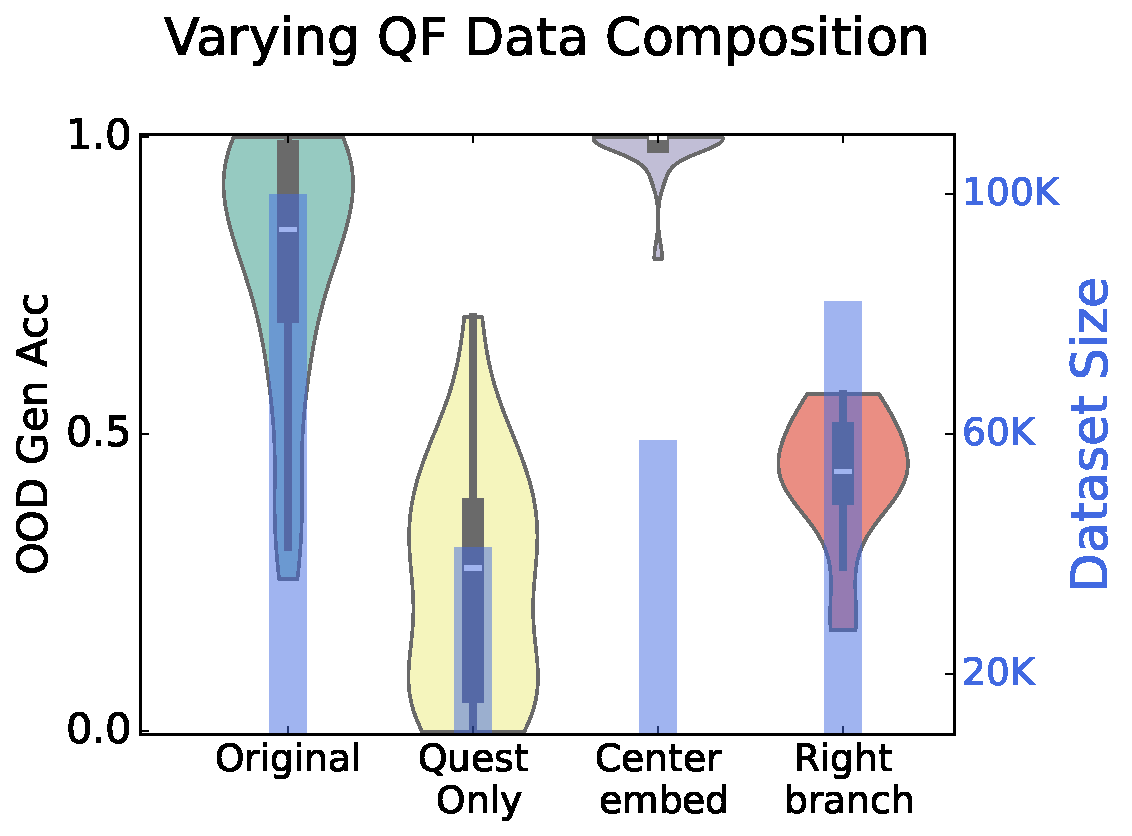
\includegraphics[width=0.41\linewidth]{figures/no_curriculum_main.pdf}
    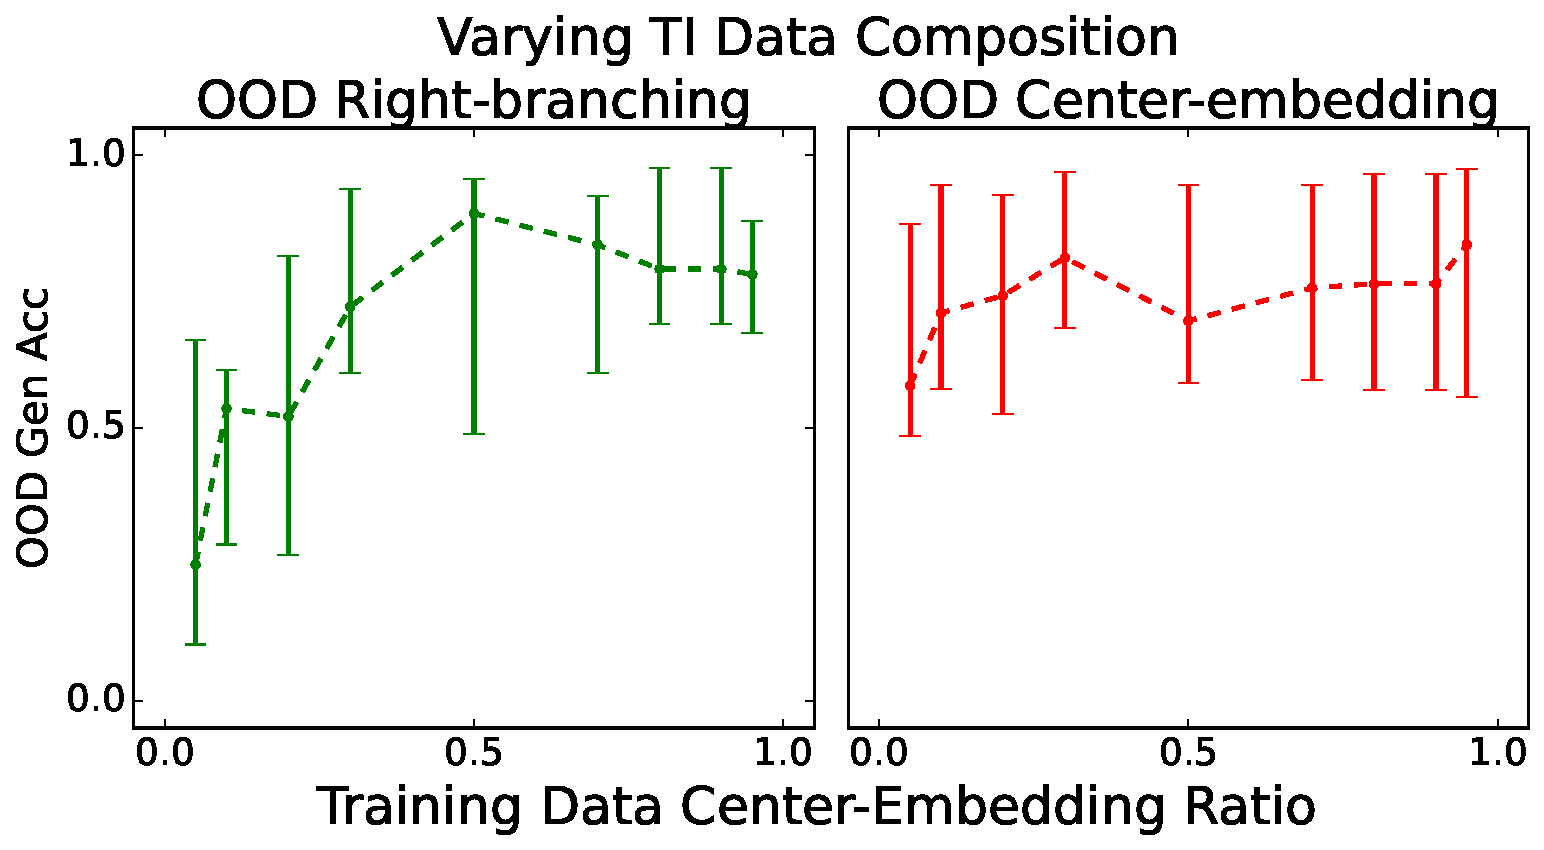
\includegraphics[width=0.55\linewidth]{figures/ti_simplicity_contamination.pdf}
    \caption{
    \textbf{Components of training data drive different generalization behaviors.} 
    \textit{Left:} Center-embedded sentences, which in the QF training data only appear in declaration copying examples, induce hierarchical generalization.
    \textit{Right:} Models are trained on different TI training data mixes and evaluated on two OOD sets: unambiguous right-branching sentences (\textit{green}) and unambiguous center-embedded sentences (\textit{red}). For center-embedded sentences, the hierarchical rule is preferred regardless of data mixes. For right-branching sentences, the model's preference for the hierarchical rule is exclusively driven by having a large mix of center-embedded sentences in the TI training data.}
    \label{fig:grokking_selection}
\end{figure}



\subsection{Tense Inflection Results}
\label{sec:ti_result}

In the TI training data, both right-branching and center-embedded sentences are made ambiguous by ensuring the distractor noun (i.e., a noun that appears between the main subject and the main verb) shares the same plurality as the main subject. For right-branching sentences, the distractor noun occurs in a prepositional phrase. For center-embedded sentences, the distractor noun occurs in a relative clause; either the subject or the object of the modifying clause can act as the distractor noun. We list examples below: 

\begin{enumerate}[itemsep=2pt,labelindent=10pt,topsep=0pt,parsep=0pt,partopsep=1pt, align=left, leftmargin=*]
    \item \textbf{Right Branching}: The noun in the prepositional phrase (e.g., `` \textit{to the cabinet}") acts as the distractor in the TI task.
    
    Example A (ID): \textit{The keys to the \textbf{cabinets} are on the table.}

    Example B (OOD): \textit{The keys to the \textbf{cabinet} are on the table.}
    
    \item \textbf{Center Embedding}: Either the subject or the object inside the relative clause acts as the distractor in the TI task.

    Example C (ID): \textit{The keys that unlock the \textbf{cabinets} are on the table.}

    Example D (OOD): \textit{The keys that unlock the \textbf{cabinet} are on the table.}
    
    
\end{enumerate}
We create variations of the TI training data by adjusting the ratio of right-branching to center-embedded samples while keeping the total training size constant.\footnote{The original training dataset contains a secondary past-tense copying task, to parallel the declaration-copying secondary task in QF. We show in Appendix \ref{appdx:ti_secondary} that the secondary task is not necessary, and we do not include it in our modified training sets.} A model's generalization behavior is tested on two OOD sets: one containing unambiguous right-branching sentences (e.g., Example B) and the other containing unambiguous center-embedded sentences (e.g., Example D). 

Generalization accuracies are shown in Figure \ref{fig:grokking_selection} (\textit{right}). When the training data is dominated by ambiguous right-branching sentences, the model fails to learn the hierarchical rule, as indicated by low OOD accuracy. However, when trained on a greater proportion of center-embedded sentences, the model systematically applies the hierarchical rule to both right-branching and center-embedded OOD sentences. As shown in Figure \ref{fig:grokking_selection} (\textit{right}), regardless of its training data mix, the model  generalizes hierarchically to OOD \textit{center embeddings}. In contrast, the model only generalizes hierarchically to \textit{right-branching sentences} after being exposed to a sufficient quantity of center-embedded sentences during training. In other words, the model eventually learns to treat non-recursive sequences as hierarchical through exposure to recursive center embeddings. These observations suggest that center embeddings drive the model's overall preference for tree structures. For further analysis of which center embedding structures induce this bias most efficiently, see Appendix \ref{appdx:obj_sbj_ctr_breakdown}.

% %%%%%%%%%%%%%%%%Previous version to preserve comments %%%%%%%%%%%%%%%%%%%%%%%%%%%%%%%%%%%%%%%%
% \iffalse
% \subsection{Tense Inflection} 
% \label{sec:ti_result}
% We now analyze hierarchical generalization in the tense inflection task, demonstrating the generality of our findings across grammatical rules. 
% The tense inflection setting from \citet{Linzen2016-vx} uses the same generation process as the question formation task, changing only the task itself.  
% This generation process leads to three types of sentences:

% \begin{enumerate}[itemsep=2pt,labelindent=10pt,topsep=0pt,parsep=0pt,partopsep=1pt, align=left, leftmargin=*]
%     \item The main verb immediately follows the subject noun.

%     Example: \textit{The keys are on the table.}
%     \item The main verb and the subject noun are separated by a prepositional phrase (e.g., `` \textit{to the cabinet}"). In all sentence examples, the prepositional phrase consistently follows the same syntactical structure and length (i.e., ``preposition $+$ determiner $+$ noun"). 

%     Example: \textit{The keys to the cabinet are on the table.}
%     \item The main verb and subject noun are separated by a relative clause, which can vary in syntactic composition and length.

%     Example: \textit{The keys that I used to unlock the cabinet are on the table.}
% \end{enumerate}


% By definition, both the first and second sentence types are right branching. In the second type, although a prepositional phrase is inserted within the main clause, it differs syntactically from a relative clause modifier. Unlike relative clause modifiers, prepositional phrases lack syntactic diversity, whereas relative clauses can exhibit the same of diversity as an entire sentence. In QF and TI data generated by CFG rules, a 4-gram model suffices to capture the subject-verb agreement. In contrast, relative clause modifiers (i.e., the third type) vary in both length and syntactic structure. All three sentence types are present in the original training data. Since sentences of the first type lack a distractor noun, they cannot be used to probe the model’s generalization, so the generalization set includes only the second and third types. As specified in Section \ref{sec:ti_task}, the TI training data only requires that the subject and distractor have the same plurality. Thus, center-embedded sentences can be included in the TI training data without violating the ambiguity requirement, and a secondary task is not necessary for TI.\footnote{In Appendix \ref{appdx:tense_tv}, we show that we can again leverage a secondary task such that a model trained on center-embedded tense inflection examples can generalize to right-branching sentences without having seen any examples of tense inflection on the sentence type, but not vice versa. }


% Our goal is to verify that center embeddings also drive OOD generalization in tense inflection. We create variations of the TI training data by adjusting the ratio of right-branching to center-embedded sentences, keeping the total training size constant. In Figure \ref{fig:ti_selection}, we report the model's OOD behavior across two data partitions. Figure \ref{fig:ti_selection} (\textit{left}) shows the model's generalization accuracy on unambiguous right-branching sentences when trained on different data mixes. When training data is dominated by ambiguous right-branching sentences, the model fails to learn the hierarchical rule, as indicated by low OOD generalization accuracy. However, as we increase the proportion of center-embedded sentences, these sentences---despite being ambiguous---bias the model towards the hierarchical rule, reflected by improved generalization accuracy.

% Figure \ref{fig:ti_selection} (\textit{right}) shows that the model consistently prefers the hierarchical rule for center-embedded sentences, regardless of data composition. These results indicate that the model’s preference for the hierarchical rule is primarily driven by center-embedded sentences. Moreover, with a high proportion of center-embedded sentences in the training data, this hierarchical rule preference extends to right-branching sentences as well.


% \fi
\subsection{Model Architecture}
\label{section:vision_model_architecture}
Our visual-recognition model consists of three main components: \textbf{(1)} an image encoder, \textbf{(2)} an image adapter, and \textbf{(3)} a video adapter.

\textbf{Image encoder.} Our image encoder is a standard vision transformer (ViT; \citet{dosovitskiy2020vit}) that is trained to align images and text \citep{xu2023demystifying}.
We use the ViT-H/14 variant of the image encoder, which has 630M parameters that were trained on 2.5B image-text pairs for five epochs.
The image encoder is pre-trained on images with resolution $224 \times 224$; images were split up into $16 \times 16$ patches of equal size (\emph{i.e.}, a patch size of $14x14$ pixels).
As also demonstrated by prior work such as ViP-Llava \citep{cai2023vipllava}, we observe that image encoders trained via a contrastive text alignment objective are unable to preserve fine-grained localization information. To alleviate this, we employ a \emph{multi-layer} feature extraction, where features from the \emph{4$^{th}$, 8$^{th}$, 16$^{th}$, 24$^{th}$ and 31$^{st}$} layers are also provided in addition to the final layer features.
In addition, we further insert 8 \emph{gated} self-attention layers (making a total of 40 transformer blocks) prior to pre-training of the cross-attention layers to learn alignment-specific features. The image encoder therefore eventually has a total $850$M parameters with the additional layers.
With the multi-layer features, the image encoder produces a $7680$-dimensional representation for each of the resulting $16 \times 16\!=\!256$ patches.
The parameters of the image encoder are \emph{not} frozen during subsequent training stages as we found it to improve performance, especially in domains such as text recognition.

\textbf{Image adapter.} We introduce cross-attention layers between the visual token representations produced by the image encoder and the token representations produced by the language model \citep{alayrac2022flamingo}.
The cross-attention layers are applied after every fourth self-attention layer in the core language model.
Like the language model itself, the cross-attention layers use generalized query attention (GQA) for increased efficiency.
The cross-attention layers introduce substantial numbers of additional trainable parameters into the model: for Llama 3 405B, the cross-attention layers have $\approx$100B parameters.
We pre-train our image adapter in two stages: (1) initial pre-training followed by (2) annealing:
\begin{itemize}
\item \textbf{Initial pre-training.} We pre-train our image adapter on our dataset of  $\sim$6B image-text pairs described above.
For compute efficiency reasons, we resize all images to fit within \emph{at most} four tiles of $336 \times 336$ pixels each, where we arrange the tiles to support different aspect ratios, \emph{e.g.}, $672 \times 672$, $672 \times 336$, and $1344 \times 336$.

\item \textbf{Annealing.}
We continue training the image adapter on $\sim$500M images from the annealing dataset described above.
During annealing, we increase the per-tile image resolution to improve performance on tasks that require higher-resolution images, for example, infographics understanding.
\end{itemize}

\textbf{Video adapter.} Our model takes as input up to 64 frames (uniformly sampled from a full video), each of which is processed by the image encoder.
We model temporal structure in videos through two components: \textbf{(i)} encoded video frames are aggregated by a temporal aggregator which merges 32 consecutive frames into one, \textbf{(ii)} additional video cross attention layers are added before every fourth image cross attention layer.
The temporal aggregator is implemented as a perceiver resampler~\citep{jaegle2021perceiver,alayrac2022flamingo}.
We pre-train using 16 frames per video (aggregated to 1 frame), but increase the number of input frames to 64 during supervised finetuning.
The video aggregator and cross attention layers have 0.6B and 4.6B parameters for Llama 3 7B and 70B, respectively. 




\subsection{Pre-training}
\label{section:vision_training_recipe}

\textbf{Image.}
We initialize from the pre-trained text model and vision encoder weights.
The vision encoder is unfrozen, while the text model weights are kept frozen as explained above.
First, we train the model using 6B image-text pairs where each image is resized to fit within four tiles of $336 \times 336$ pixels.
We use a global batch size of 16,384 and a cosine learning rate schedule with initial learning rate $10 \times 10^{-4}$ and a weight decay of $0.01$.
The initial learning rate was determined based on small-scale experiments.
However,  these findings did not generalize well to very long training schedules and dropped the learning rate a few times during training when the loss values became stagnant.
After the base pre-training, we increase the image resolution further and continue training the same weights on the annealing dataset.
The optimizer is re-initialized via warm-up to learning rate $2 \times 10^{-5}$ and again follows a cosine schedule.

\textbf{Video.}
For video pre-training, we start from the image pre-trained and annealed weights as described above.
We add the video aggregator and cross-attention layers as described in the architecture, initialized randomly. We freeze all the parameters in the model except the video-specific ones (the aggregator and video cross-attention), and train them on the video pre-training data.
We use the same training hyperparameters as the image annealing stage, with small differences in the learning rate.
We uniformly sample 16 frames from the full video, and represent each frame using four chunks, each of size of $448 \times 448$ pixels.
We use an aggregation factor of 16 in the video aggregator, hence obtaining one effective frame, which the text tokens cross-attend to.
We use a global batch size of 4,096, a sequence length of 190 tokens, and a learning rate of $10^{-4}$ during training.



\subsection{Speech Understanding Results}
\label{section:results_speech}
We evaluate the speech understanding capabilities of our speech interface for Llama 3 on three tasks: \textbf{(1)} automatic speech recognition, \textbf{(2)} speech translation, and \textbf{(3)} spoken question answering.
We compare the performance of our speech interface for Llama 3 with three state-of-the-art models for speech understanding: Whisper \citep{radford23whisper}, SeamlessM4T \citep{barrault2023seamless}, and Gemini.\footnote{
	Due to technical limitations, we compare with the performance of Gemini on MLS reported in the original paper.
}
In all the evaluations, we used greedy search for Llama 3 token prediction.

\textbf{Speech recognition.}
We evaluate the ASR performance on the
English datasets of
Multilingual LibriSpeech (MLS; \citet{pratap2020mls}),
LibriSpeech \citep{panayotov2015librispeech},
VoxPopuli \citep{wang2021voxpopuli},
and a subset of the multilingual FLEURS dataset \citep{conneau2023fleurs}.
In evaluation, the decoding results are post-processed using the Whisper text normalizer to ensure consistency in comparing with the reported results of other models.
On all benchmarks, we measure the word error rate of our speech interface for Llama 3 on the standard test set of those benchmarks, except for Chinese, Japanese, Korean and Thai, where the character error rate is reported.



\providecommand{\bup}{($\boldsymbol\uparrow$)}
\providecommand{\bdown}{($\boldsymbol\downarrow$)}


\begin{table}[t]
	\centering
	 \resizebox{\linewidth}{!}{\begin{NiceTabular}{lcccccc}
	\CodeBefore
	\Body
	\toprule
	& \textbf{Llama 3 8B} & \textbf{Llama 3 70B} & \textbf{Whisper} & \textbf{SeamlessM4T v2} & \textbf{Gemini 1.0 Ultra} & \textbf{Gemini 1.5 Pro}\\
	\midrule
	MLS \scriptsize{(English)} & 4.9 & 4.4 & 6.2 \scriptsize{(v2)} & 6.5 & 4.4 & \textbf{4.2} \\
	LibriSpeech \scriptsize{(test-other)} & 3.4 & \textbf{3.1} & 4.9 \scriptsize{(v2)} & 6.2 & -- &  -- \\
	VoxPopuli \scriptsize{(English)}  & 6.2 & \textbf{5.7} &  7.0  \scriptsize{(v2)} & 7.0 & -- & --  \\
	FLEURS \scriptsize{(34 languages)} & 9.6 & \textbf{8.2} & 14.4 \scriptsize{(v3)}  & 11.7 & -- & -- \\
	\bottomrule
\end{NiceTabular}
}
	\caption{\textbf{Word error rate of our speech interface for Llama 3 on speech recognition tasks.} We report the performance of Whisper, SeamlessM4T, and Gemini for reference.}
	\label{table:speech_asr_results}
\end{table}


Table~\ref{table:speech_asr_results} shows the results of ASR evaluations.
It demonstrates the strong performance of Llama 3 (and multi-modal foundation models more generally) on speech recognition tasks: our model outperforms models that are tailored to speech like Whisper\footnote{On FLEURS ASR, Malayalam is not officially reported for Whisper v3, so we use the average of 33 languages.} and SeamlessM4T on all benchmarks.
On MLS English, Llama 3 performs similarly to Gemini.


\begin{table}[t]
	\centering
	\begin{NiceTabular}{lcccc}
	\CodeBefore
	\Body
	\toprule
	& \textbf{Llama 3 8B} & \textbf{Llama 3 70B} & \textbf{Whisper v2} & \textbf{SeamlessM4T v2}\\
	\midrule
	FLEURS \scriptsize{(33 lang. $\rightarrow$ English)} & 29.5 & \textbf{33.7}  & 21.9  & 28.6  \\
	Covost 2 \scriptsize{(15 lang. $\rightarrow$ English)} & 34.4 & \textbf{38.8} & 33.8  & 37.9 \\
	\bottomrule
\end{NiceTabular}

	\caption{\textbf{BLEU score of our speech interface for Llama 3 on speech translation tasks.} We report the performance of Whisper and SeamlessM4T for reference.}
	\label{table:speech_ast_results}
\end{table}


\textbf{Speech translation.}
We also evaluate our models on speech translation tasks in which the model is asked to translate non-English speech into English text.
We use the FLEURS and Covost 2 \citep{wang2021covost} datasets in these evaluations, measuring BLEU scores of the translated English.
Table~\ref{table:speech_ast_results} presents the results of these experiments.\footnote{On Covost 2, we evaluate only on 15 (out of 21) languages.} 
The performance of our models in speech translation highlights the advantages of multimodal foundation models for tasks such as speech translation. 

\begin{figure}[]
    \centering
    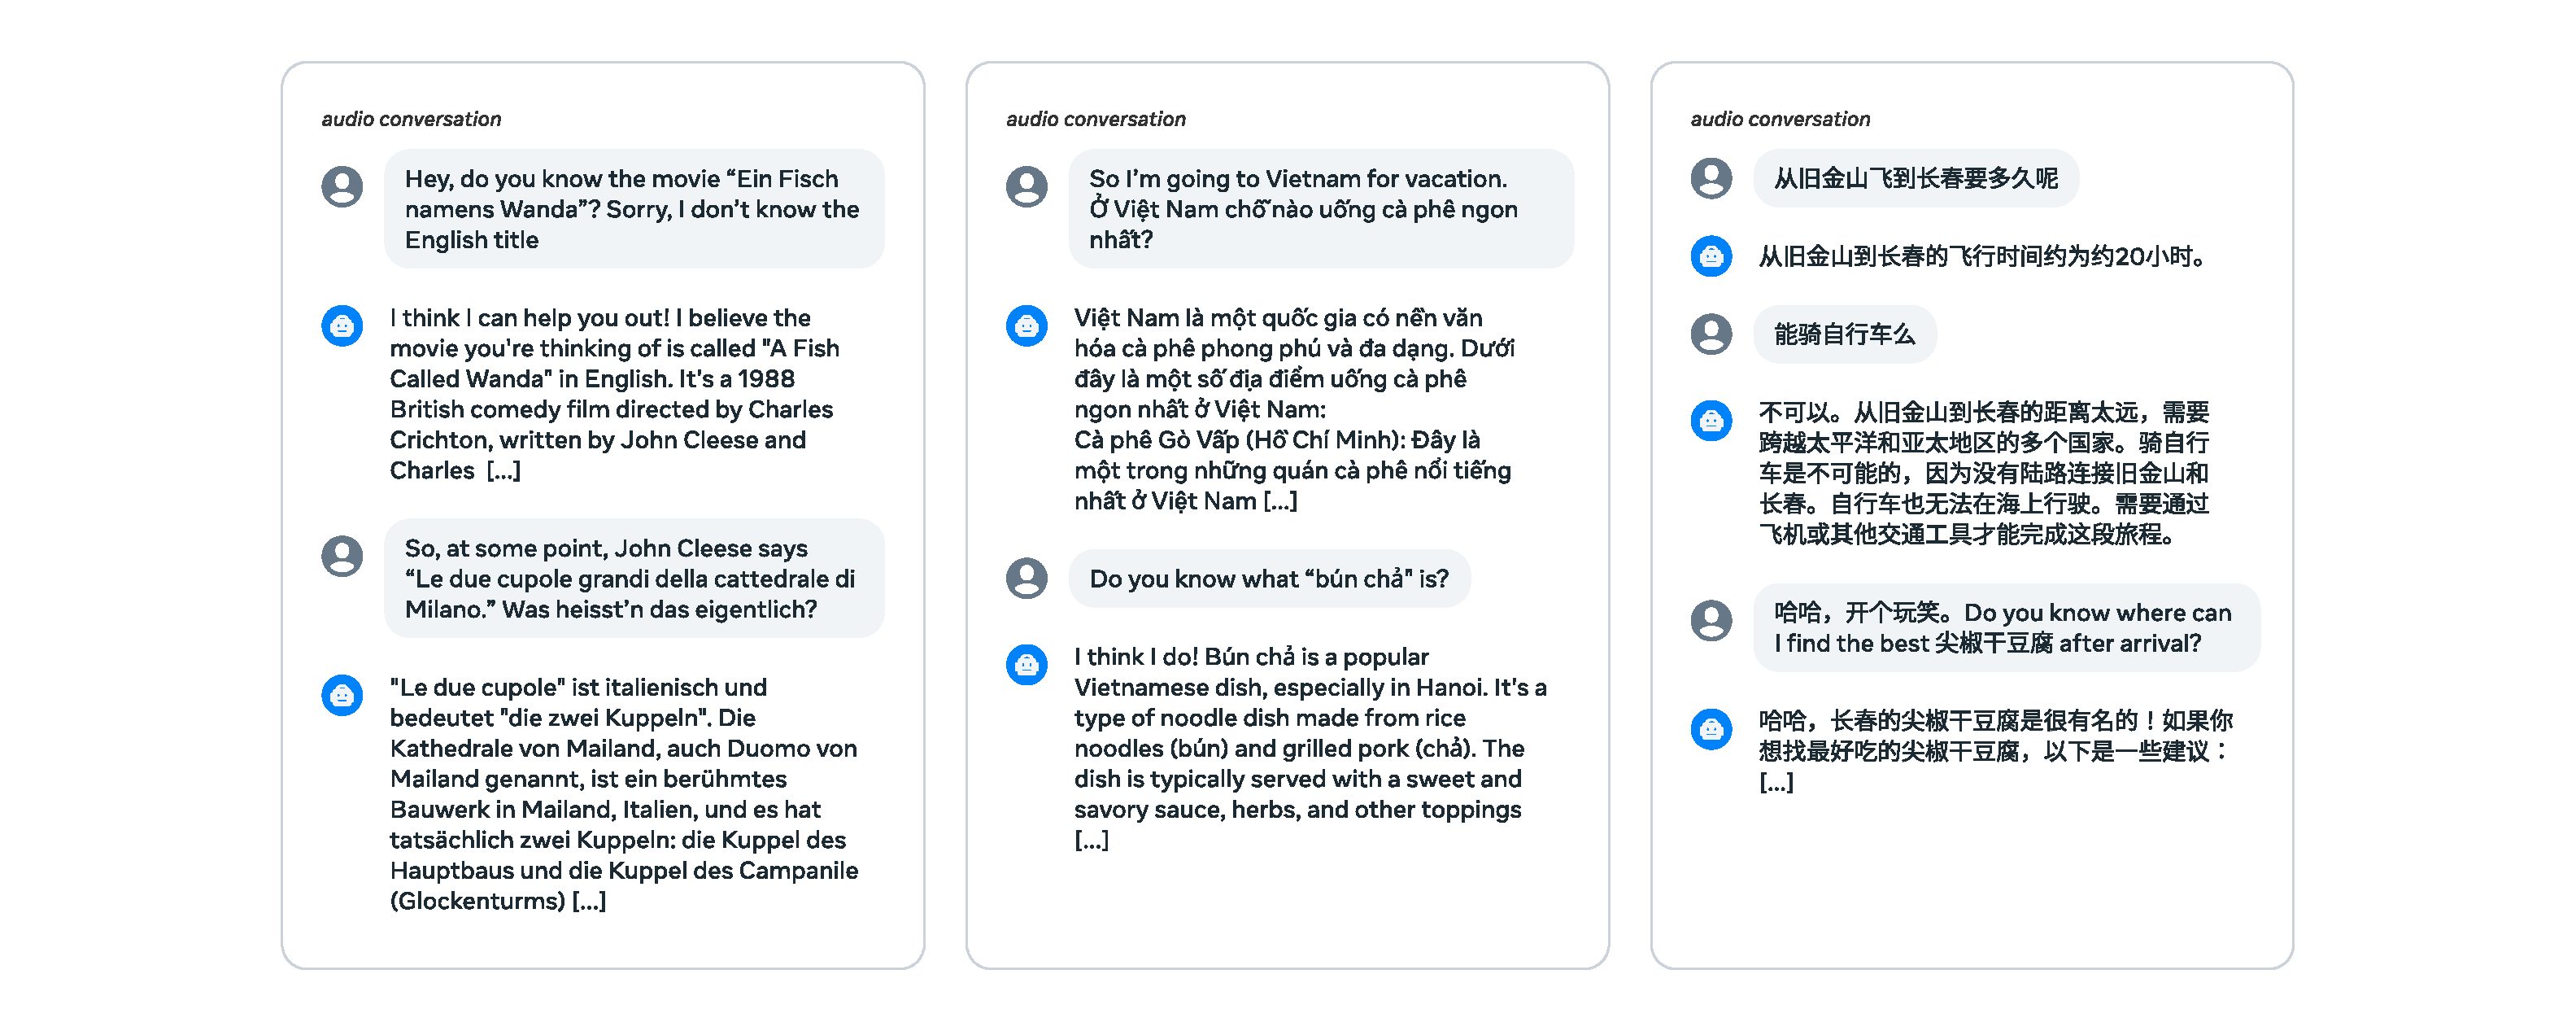
\includegraphics[trim={150px 0 150px 0},clip,width=\textwidth]{assets/llama-voice-language.pdf}
    \caption{\textbf{Transcribed dialogue examples using the speech interface for Llama 3.} The examples illustrate zero-shot multi-turn and code-switching capabilities.}
    \label{figure:speech_dialog_example}
\end{figure}

\textbf{Spoken question answering.}
The speech interface of Llama 3 demonstrates remarkable question answering capabilities. The model can effortlessly comprehend code-switched speech without any prior exposure to such data. Notably, although the model was trained only on single-turn dialogue, it is capable of engaging in extended, coherent multi-turn dialogue sessions.
Figure~\ref{figure:speech_dialog_example} presents a few examples that highlight these multilingual and multi-turn capabilities.

\begin{table}[t]
\centering
    \begin{tabular}{lcccccc}
    \toprule
     & \multicolumn{2}{c}{\textbf{Llama 3 8B}} &  \multicolumn{2}{c}{\textbf{Llama 3 70B}} & \multicolumn{2}{c}{\textbf{Gemini 1.5 Pro}} \\
    \textbf{Language} & AT \bdown & LT \bup & AT \bdown & LT  \bup & AT \bdown & LT \bup \\
    \midrule
    English & 0.84 & 15.09 & \textbf{0.68} & \textbf{15.46} & 1.44 & 13.42 \\
    Overall & 2.31 & 9.89 & \textbf{2.00} & 10.29 & 2.06 & \textbf{10.94} \\
    \bottomrule
    \end{tabular}
    \caption{\textbf{Speech toxicity of our speech interface to Llama 3 on the MuTox dataset.} AT refers to added toxicity (\%) and LT refers to lost toxicity (\%). \label{table:speech-safety-mutox}}
\end{table}

\textbf{Safety.}
We evaluate the safety of our speech model on MuTox \citep{mutox}, a multilingual audio-based dataset of 20,000 utterances for English and Spanish and 4,000 for 19 other languages, each with toxicity labels attached.
The audio is passed as input to the model and the output is evaluated for toxicity, after cleaning some special characters.
We apply the MuTox classifier~\citep{mutox} and compare the results with Gemini 1.5 Pro. We evaluate the percentage of added toxicity (AT), when the input prompt is safe and the output is toxic, and the percentage of lost toxicity (LT), when the input prompt is toxic and the answer is safe. Table~\ref{table:speech-safety-mutox} shows the results for English and an average across all 21 languages that we evaluated on.\footnote{Note that for Gemini, we encountered that a significant number of responses were empty, which could be due to safety filters on their side (though some empty responses were for non-toxic input) or to rate limits. To conduct the analysis, we assumed that all the empty responses are safe. This is the most conservative approach for results and the upper bound of what Gemini results would look like.} The percentage of added toxicity is very low: our speech models have the lowest percentage of added toxicity for English, with less than 1\%. It removes significantly more toxicity than it adds.


\subsection{Speech Generation Results}
For speech generation, we focus on evaluating the quality of token-wise input streaming models with the Llama 3 embeddings for the text normalization and prosody modeling tasks. The evaluation focuses on comparisons with models that do not take the Llama 3 embeddings as an additional input.

\textbf{Text normalization.}
To measure the effect of Llama 3 embeddings, we experimented with changing the amount of right context the model uses. We trained the model using a right context of 3 TN tokens (demarcated by unicode category). This model is compared to models that do not use the Llama 3 embeddings, using a 3-token right context or a full bi-directional context.
As expected, Table~\ref{tab:table1} shows using the full right context improves performance for the model without Llama 3 embeddings. However, the model that incorporates the Llama 3 embeddings outperforms all other models, hence enabling token-rate input/output streaming without relying on long context in the input.

\begin{wraptable}{r}{0.45\textwidth}
	\begin{NiceTabular}{lcc}
		\CodeBefore
		\Body
		\toprule
		\textbf{Model} & \textbf{Context} & \textbf{Accuracy} \\
		\midrule
		Without Llama 3 8B & 3 & 73.6\% \\
		Without Llama 3 8B & $\infty$ & 88.0\% \\
		With Llama 3 8B & 3 & \textbf{90.7\%} \\
		\bottomrule
	\end{NiceTabular}
	\caption{\textbf{Sample-wise text normalization (TN) accuracy.} We compare models with or without Llama 3 8B embeddings, and using different right-context values.\vspace{-8mm}}
	\label{tab:table1}
\end{wraptable}

\textbf{Prosody modeling.}
To evaluate the performance of the our prosody model (PM) with Llama 3 8B, we conducted two sets of human evaluation comparing models with and without Llama 3 embeddings. Raters listened to samples from different models and indicated their preferences. To generate the final speech waveform, we use an in-house transformer based acoustic model \citep{wu2021transformer} that predicts spectral features and a WaveRNN neural vocoder \citep{kalchbrenner2018efficient} to generate the final speech waveform.  %

\begin{table}[t]
	\centering
    \begin{minipage}{.48\textwidth}
      \centering
      \begin{tabular}{lcc}
		\toprule
		\textbf{Model} & \textbf{Preference} \\
		\midrule
		PM for Llama 3 8B  & \textbf{60.0\%} \\
		\small{Streaming phone-only baseline} & 40.0\% \\
		\bottomrule
      \end{tabular}
		\label{tab:tts:pm:ab_test1}
    \end{minipage}\hfill
    \begin{minipage}{.48\textwidth}
      \centering
      \begin{tabular}{lcc}
		\toprule
		\textbf{Model} & \textbf{Preference} \\
		\midrule
		PM for Llama 3 8B & \textbf{63.6\%} \\
		\small{Non-streaming phone-only baseline} & 36.4\% \\
		\bottomrule
      \end{tabular}

    \end{minipage}
    \caption{\textbf{Prosody Modeling (PM) evaluation.} \emph{Left:} Rater preferences of PM for Llama 3 8B vs. streaming phone-only baseline. \emph{Right:} Rater preferences of PM for Llama 3 8B vs. non-streaming phone-only baseline.}
    \label{tab:pm_test}

\end{table}




First, we compare directly to a streaming baseline model without Llama 3 embeddings. 
In  the second test, the Llama 3 8B PM is compared to a non-streaming baseline model without Llama 3 embeddings. 
As shown in Table~\ref{tab:pm_test}, the Llama 3 8B PM is preferred  60\% of the time compared to the streaming baseline, and 63.6\% of the time  compared to the non-streaming baseline, indicating a significant improvement in perceived quality. The key advantage of the Llama 3 8B PM is its token-wise streaming capability (Section~\ref{sec:tts:pm}), which maintains low latency during inference. This reduces the model's lookahead requirements, enabling more responsive and real-time speech synthesis compared to non-streaming baselines.
Overall, the Llama 3 8B prosody model consistently outperforms the baseline models, demonstrating its effectiveness in enhancing the naturalness and expressiveness of synthesized speech.

